%%% template.tex
%%%
%%% This LaTeX source document can be used as the basis for your technical
%%% paper or abstract. Intentionally stripped of annotation, the parameters
%%% and commands should be adjusted for your particular paper - title,
%%% author, article DOI, etc.
%%% The accompanying ``template.annotated.tex'' provides copious annotation
%%% for the commands and parameters found in the source document. (The code
%%% is identical in ``template.tex'' and ``template.annotated.tex.'')

\documentclass[]{acmsiggraph}
\usepackage{algorithm}
\usepackage[noend]{algpseudocode}
\TOGonlineid{45678}
\TOGvolume{0}
\TOGnumber{0}
\TOGarticleDOI{0}
\TOGprojectURL{}
\TOGvideoURL{}
\TOGdataURL{}
\TOGcodeURL{}
\usepackage{color}
%\definecolor{red}{rgb}{0.9, 0.17, 0.31}
\usepackage{multirow}
\usepackage{subfig}
\usepackage{xcolor}
\usepackage{lipsum}
\usepackage{listings}
\usepackage{graphicx}
\usepackage{glsllst} % My own package providing markup listing for glsl
\usepackage{rmlst}   % My own package providing markup listing for renderman
\usepackage{amsmath}
\usepackage{hyperref}
\usepackage{underscore}

\lstset{
	backgroundcolor=\color[rgb]{0.95, 0.95, 0.95},
	tabsize=3,
	%rulecolor=,
	basicstyle=\footnotesize\ttfamily,
	upquote=true,
	aboveskip={1.5\baselineskip},
	columns=fixed,
	showstringspaces=false,
	extendedchars=true,
	breaklines=true,
	prebreak = \raisebox{0ex}[0ex][0ex]{\ensuremath{\hookleftarrow}},
	frame=none,
	aboveskip=15pt,
	belowskip=8pt,
	captionpos=t,
	showtabs=false,
	showspaces=false,
	showstringspaces=false,
	identifierstyle=\ttfamily,
	%keywordstyle=\color{red}\bfseries,
	%keywordstyle=[1]\bfseries\color{syntaxBlue},
	%keywordstyle=[2]\bfseries\color{syntaxRed},
	%keywordstyle=[3]\color{blue}\bfseries,
	%keywordstyle=[4]\bfseries\color{syntaxBlue},
	commentstyle=\color[rgb]{0.082,0.639,0.082},
	keywordstyle=[1]\bfseries\color[rgb]{0,0,0.75},
	keywordstyle=[2]\bfseries\color[rgb]{0.5,0.0,0.0},
	keywordstyle=[3]\bfseries\color[rgb]{0.127,0.427,0.514},
	keywordstyle=[4]\bfseries\color[rgb]{0.4,0.4,0.4},
	stringstyle=\color[rgb]{0.639,0.082,0.082},
}

\title{Simulation Techniques for Animation: GPU Accelerated Mass Spring System}

\author{Joe Withers\thanks{e-mail:joewithers96gmail.com}}
\pdfauthor{Joe Withers}

\keywords{simulations}

\begin{document}

%% \teaser{
%%   \includegraphics[height=1.5in]{images/sampleteaser}
%%   \caption{Spring Training 2009, Peoria, AZ.}
%% }

\maketitle

\begin{abstract}
During this project I explored the feasibility of offloading computation onto the GPU, in soft body Mass-spring system simulations, focusing primarily on techniques that make use of OpenGL compute shaders. This report documents my implementation of such techniques, as well as my findings.
\end{abstract}
%\keywordlist
%\TOGlinkslist


\section{Implementation} \label{sec:implementation}

\subsection{Introduction}

Mass spring Systems are a method of approximating deformation by discretizing the the geometry into a series of masses, that are connected by deformable springs. Masses in these systems are commonly arranged in a cartesian axis aligned grid, as shown in Figure~\ref{fig:springs}. Varying the dimensions of the grid allows the system to approximate different objects, such as hair strands (1 dimensional), sections of cloth (2 dimensional), or soft body 'jello' cubes (3 dimensional).

Aside from hair and cloth simulations, mass-spring systems are also used for medical purposes, such as in surgical simulations \cite{surgical}. For my implementation I have focused on the 3 dimensional case, a 'jello' cube.

\subsection{Resources}
I used C++ and OpenGL to develop my implementation, utilising the NCCA Graphics Library NGL \cite{ngl} to interact with OpenGL, and Qt5 to create the user interface. I based my implementation around a demo of a Mass-spring System using RK4 (Runge-Kutta 4th Order) integration \cite{nglMassSpring}, that uses NGL and Qt5 for it's user interface. I was able to use many aspects this implementation as 'boilerplate code', such as the camera movement and passing of basic geometry to OpenGL, which saved me a lot of time and allowed me to focus on developing the simulation itself. This implementation also provided an example of RK4 integration and calculations of spring forces according to Hooke's law, though these needed to be altered to make them suitable for use with GPU computation.

\subsection{Data Structures}

Before starting to implement the system on the GPU, I first had to establish what the data structures for the mass-spring system would be, and to do this I looked at tutorial material covering game physics systems \cite{gafferPhys} hosted by Gaffer On Games. This provided me with an understanding of the necessary data I would need to store for each mass object in the system. I determined that each mass object would be a struct of two vectors:

\begin{itemize}
	\item \lstinline{Vec3} Position - This stores the position of the mass in world space coordinates.
	\item \lstinline{Vec3} Velocity - This stores the combined speed and direction at which the mass is travelling.
\end{itemize}

To determine the data required to represent the springs I looked at tutorial material covering implementations of spring physics in game engines \cite{gafferSpring}, hosted by Gaffer On Games. This article explains that the calculation of damped spring forces, according to Hooke's law, can be calculated by following:

\begin{equation}
	F = -k(|x|-d)(x/|x|) - bv \\
\end{equation}
where:

% \begin{center}
$F$ = The force to apply to each of the mass points. \\
$k$ = The spring constant. \\
$|x|$ = The distance between the two mass points. \\
$d$ = The resting length of the spring. \\
$b$ = The damping coefficient for the spring. \\
$v$ = The relative velocity between the spring points. \\
% \end{center}
I then determined that the data for the spring object could be represented with the following struct:
\begin{itemize}
	\item \lstinline{unsigned int} Start Index - This stores an integer that represents one of the connected masses, as an index into the array of masses.
	\item \lstinline{unsigned int} End Index - This stores an integer that represents the other connected mass, as an index into the array of masses.
	\item \lstinline{float} Resting Length - This stores the original resting length of the spring.
	\item \lstinline{Vec3} Relative Velocity - This stores the combined speed and direction at which the masses are travelling to or from each other.
\end{itemize}

\subsection{GPU Computation}

For my first attempt at GPU implementation I decided to store each the attributes for each mass struct and each spring struct in OpenGL textures, similar to the technique used in \cite{massSpringGPU}, but to use Image Load/Store commands for accessing and manipulating data. The following attributes would need to be stored as 1D textures:

\begin{itemize}
	\item Mass positions - \lstinline{Vec3, RGBA32F}, Size = Number of Masses.
	\item Spring velocity - \lstinline{Vec3, RGBA32F}, Size = Number of Springs.
	\item Spring resting length - \lstinline{float, R32F}, Size = Number of Springs.
	\item Spring start index - \lstinline{unsigned int, R16UI}, Size = Number of Springs.
	\item Spring end index - \lstinline{unsigned int, R16UI}, Size = Number of Springs.
\end{itemize}

To initialise these textures, I first dispatch a compute shader with workgroups equal to the dimensions of my ‘JelloCube’ object. This sets the initial position for the masses in the mass positions texture, whilst also counting how many springs need to be created using an atomic counter. The masses are arranged in a cartesian axis aligned grid, with three different types of springs connecting them: structural, shear, and bending. Figure~\ref{fig:springs} provides a diagram of the connectivity between springs and their masses.

\begin{figure}[t]
\centering
\subfloat[Structural Springs]{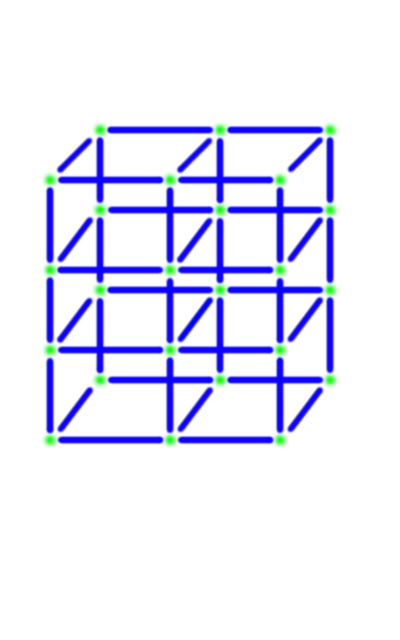
\includegraphics[width=0.15\textwidth]{images/structural.png}}
\subfloat[Shear Springs]{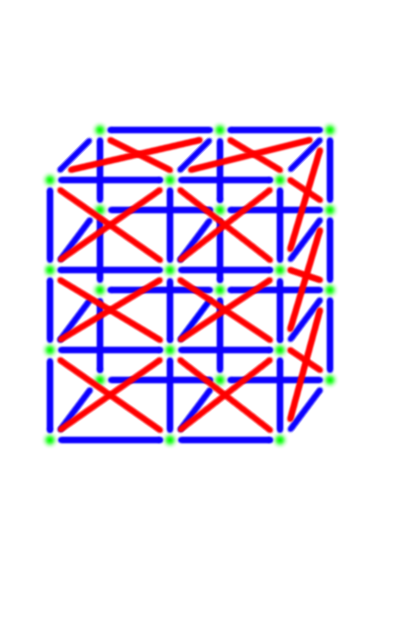
\includegraphics[width=0.15\textwidth]{images/shear.png}}
\subfloat[Bending Springs]{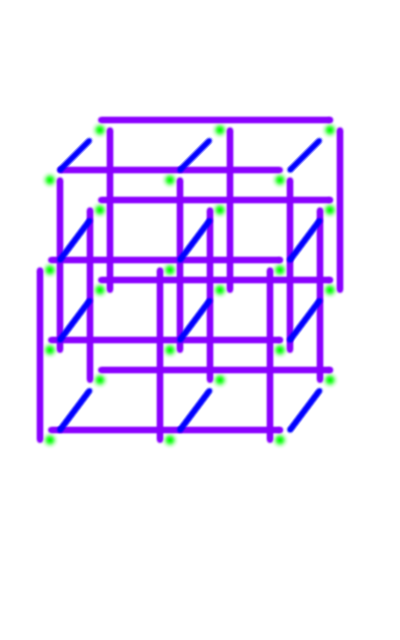
\includegraphics[width=0.15\textwidth]{images/bend.png}}
\caption{Diagrams showing the connectivity of each type of spring and their masses. \protect\cite{siggraphPixar}}
\label{fig:springs}
\end{figure}

I then read the contents of atomic counter and create the textures necessary for spring attributes, whose length is equal to the number of springs counted by the atomic counter. The atomic counter is then reset, and the compute shader is then dispatched for a second time, however this time it calls a subroutine which stores the spring attributes into each corresponding texture.

Whilst this approach works, it relies on maintaining six textures at once, which is quite unwieldy. I also found that once the number of masses is increased past 1000, the number of springs needed to be stored exceeds the number of texels I can specify with glTexImage1D, at least on my system. I therefore decided to switch to using Shader Storage Buffer Objects, as their size is only limited by the amount of memory on the GPU, and they are much easier to maintain and manipulate compared to textures.

Shader Storage Buffer Objects allow the passing of structs to directly shaders, so I was able to reduce my system to using just two Shader Storage Buffer Objects; One stores an array of Mass structs, the other stores an array of Spring structs. Upon changing the system to use Shader Storage Buffer Objects, I found them to be much faster, allowing up to 1.5 million springs to be calculated at once with interactive framerates.

Spring calculations are then performed by dispatching a compute shader two times. The first dispatch performs RK4 integration to calculate the updated relative velocity for the each of the springs. The second dispatch makes use of the \textit{NV_shader_atomic_float} extension to allow atomic operations to be used with 32 bit floats, which is used to accumulate the calculated velocity onto each of the positions of each of the mass points, in parallel.

\subsection{Physics Calculations} \label{sec:physics}

I then attempted to implement gravity and collisions with the ground plane, by adding an additional 'external forces' compute shader pass which operates on each mass, after the spring computation pass. This compute shader accumulates velocity towards the ground plane, and performs basic collision detection by clamping the mass position Y coordinate to 0, and reflecting the velocity Y value should the mass position be below the ground plane. I found this to be unsuccessfull as the spring forces were not able to counteract the velocity accumulated by 'gravity', resulting in the system being unable to achieve a resting position on the plane. I then attempted to accumulate the mass velocity in the spring calculation pass, however this resulted in the masses oscillating uncontrollably.

In reading the notes from a Pixar presentation about GPU compute \cite{siggraphPixar}, I found a solution; extend the mass struct to store a 'Force' value, which the output of the spring calculation pass can then be accumulated on. The 'external forces' compute shader pass can then accumulate gravity onto this value, and use it to calculate the updated mass velocity. The 'Force' value is then cleared before starting the spring computation pass again for the next time step. This was also beneficial as it allowed me to apply 'Forces' directly upon detecting collision. Slight instability was still present, but I was able to mitigate it by introducing pseudo air resistance, which simply multiplies the velocity by a fixed value (0.99 for example).

I then implemented additional physics interactions, such as collision with a sphere, friction, and a constant for restitution or 'recovery'. Collisions with the sphere are handled in the 'external forces', and uses signed distance to determine whether a mass is inside the sphere. If it determines the mass is within the sphere, it projects the position of the mass onto the surface of the sphere, and applies force to the mass in the direction of the normal on that point on the surface. Friction is applied by multiplying the mass velocity by a fixed constant if collision is detected. Restitution is implemented by updating the spring's resting length with a value that is linearly interpolated between the resting length and the current distance between the masses. In reading an article explaining the use of restitution coefficients in mass-spring systems \cite{restitution}, I realised that this method does not account for the transfer of kinetic energy, so will likely result in inaccurate behaviour.

One of the features I had planned initially was the ability to choose between RK4, RK2, and Euler integration. As I had already implemented RK4, it was relatively simple to implement RK2 and Euler methods, though I referred to example implementations \cite{integrators} to ensure my calculations were correct.

\section{Research Report} \label{sec:report}

\subsection{Materials}

Whilst performant, I didn't find the techniques described in \textit{Mass-Spring Systems on the GPU} \cite{massSpringGPU} to be ideal for my implementation as it requires maintaining multiple textures for each of the attributes in the mass-spring system. Fortunately, Shader Storage Buffer Objects have been implemented in OpenGL since the paper was written, allowing me to pass data almost arbitrarily between compute shader stages. Another advantage of using Shader Storage Buffer Objects is that they can be sized up to the limit of GPU memory, writen to atomically, allowing parallel manipulation of data, and structs can be passed from the host program to the GPU with relative ease.

This allowed me to use a technique similar to the one described in \cite{siggraphPixar}, which makes use of CUDA to perform mass-spring simulations with RK4 integration, by sending the required data to the GPU via structs. Aside from using OpenGL compute shaders rather than CUDA, my implementation is notably different from the one descibed here, as my integration step only evaluates the forces exerted by the springs. The data structures used in \cite{siggraphPixar} store additional velocity values, one for each evaluation in the RK4 integration, allowing both spring forces and external forces to be accounted for in the integration. This results in improved collision detection behaviour when compared to my implementation, however the issue is somewhat mitigated by the fact that I do not simulate self collisions within the mass-spring system, nor do I simulate collisions between multiple mass-spring systems.

\subsection{Results}

Overall I was quite impressed by the performance I was able to gain by offloading the physics calculations for my system onto the GPU. I am able to maintain interactive framerates with all of the aforementioned physics calculations being performed 10 times a frame, on an object with 1000 masses and 9960 springs. GPU memory usage is also remarkably low at just 70MiB.

Whilst my implementation may not be physically accurate, the performance results are comparable to other GPU Mass Spring System implementations, such as those described in \cite{massSpringGPU} and \cite{siggraphPixar}. Figure~\ref{fig:screenshots} shows screen captures of my implementation.

\begin{figure}[htbp]
	\centering
	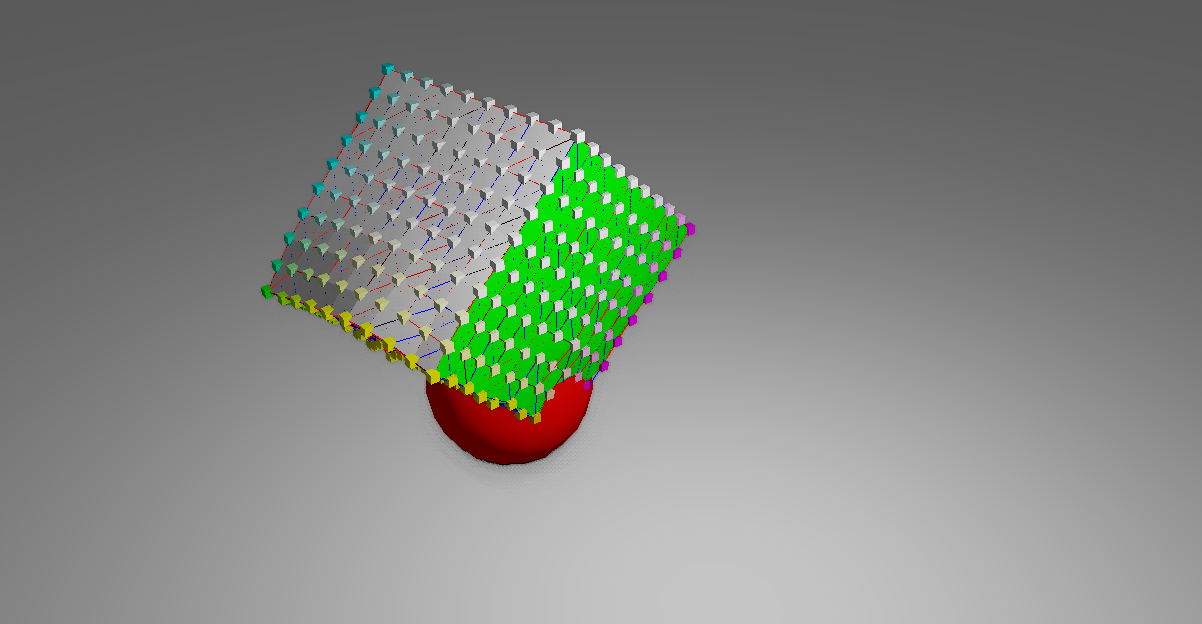
\includegraphics[width=0.9\linewidth]{images/screenshot001.png}
	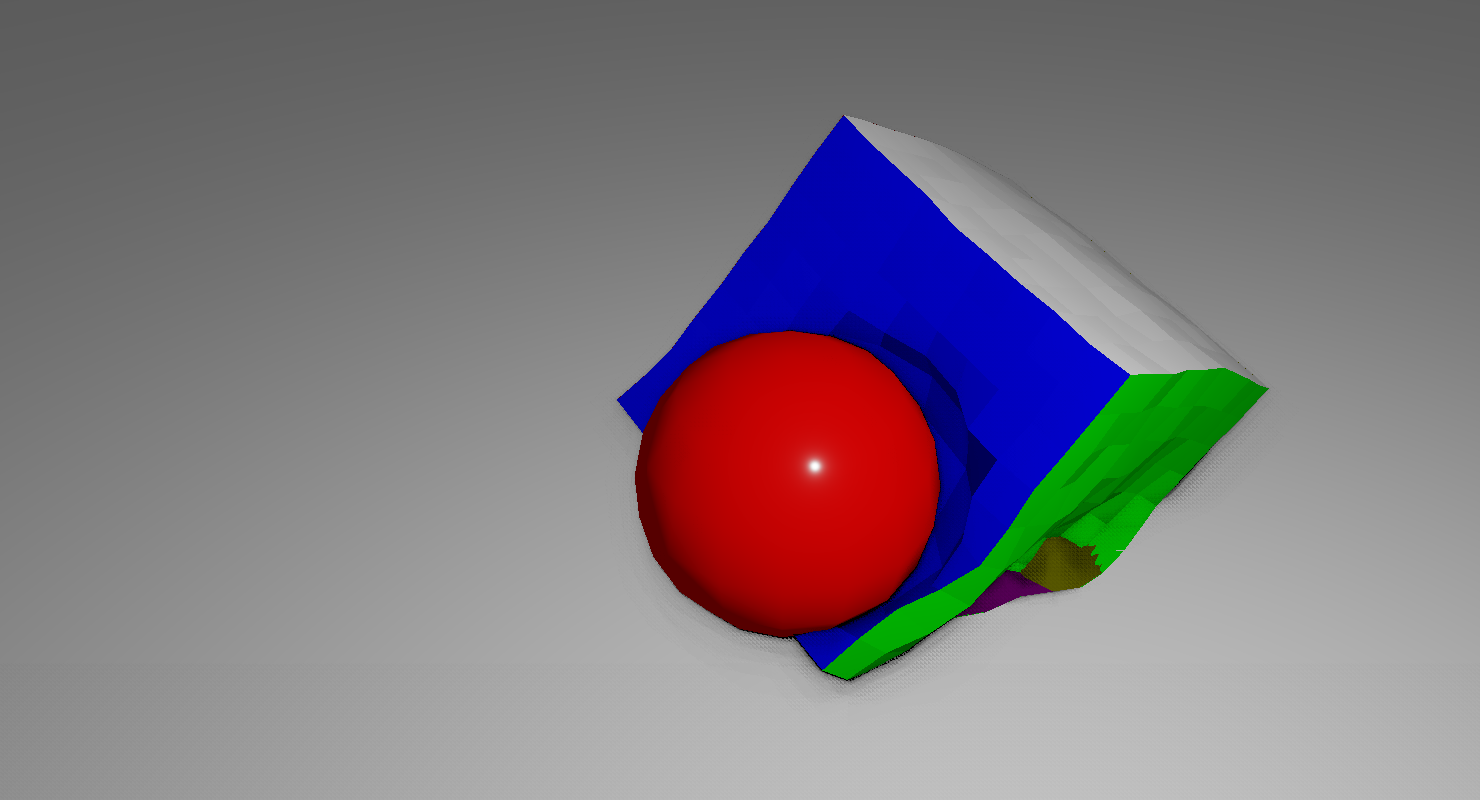
\includegraphics[width=0.9\linewidth]{images/screenshot002.png}
	\caption{\label{fig:screenshots} Screenshots of my implementation showing collision with a moving sphere, and the resulting  deformation.}
\end{figure}

Towards the end of the assignment I was able to implement a simple physically based shading model, and screen-space ambient occlusion. Whilst these may seem like novelty features, they greatly improve the usability of the system as it becomes much easier to 'read' the spatial properties of the scene, and indicates areas of geometry that are colliding or nearing collision.

\subsection{Improvements}

Whilst I am pleased with the performance of my implemetation, there are however a number of problems within my physics calculations that reduce the overal quality of my simulation.

One thing I have noticed is that, although I have implemented the option to switch between different integration schemes, the difference between them is negligible. I suspect this is because I am using very small timestep, and have also implemented 'sub steps', which performs the physics calculations multiple times per frame at even smaller timestep values. An article \cite{integrators} I looked at whilst researching integrators notes that the error present in Euler integration can be reduced by running the integration multiple times at smaller time steps, which would seem to confirm this. I could also consider implementing Verlet integration, as used in \cite{massSpringGPU}, however this would require storing additional variables for the previous mass positions and velocities.

In my final implementation there are sometimes errors in which the collision detection doesn't evaluate correctly, and the sphere is able to pass through the object. I believe this is due to the fact that numerical integration is only performed in the spring calculation pass, and not in the external forces pass. Therefore it only evaluates the forces from the springs within the integrator, and not the forces applied by gravity or collisions. Fixing this would require heavy restructuring of my implementation, though it would be necessary for a more accurate implementation.

As mentioned in Section~\ref{sec:physics}, the calculation used for simulating restitution is not physically plausible, as it does not account for the transfer of kinetic energy into the spring. This results in gradual 'squashing' of the system under gravitational force if the recovery value is set to anything less than $1.0$.

\bibliographystyle{acmsiggraph}
\bibliography{references}

\end{document}
